\rule{0.5\textwidth}{0.5pt}\\

	{\large \textbf{EXPERIMENT CroppedBNFC10000-1}}\\
	
	{\normalsize HYPERPARAMETERS:}
	\begin{lstlisting}	
	*ARCHITECTURE HYPERPARAMETERS:
		-Fully Connected
		-Input shape: 19
		-Output shape: 8192
		-Hidden layers: [1024, 1024, 1024, 1024, 1024, 1024]
		-Regularizer: None
		-Hidden Layers Activation: relu
		-Output Layer Activation: linear
		-Batch Normalization: True
		-Dropout: False, 0.2
	
	*COMPILATION HYPERPARAMETERS:
		-Optimizer: ADAM lr=0.0001, beta_1=0.9, beta_2=0.999
		-Loss Function: MSE
		-Metric: MSE
	
	*TRAINING HYPERPARAMETERS:
		-Epochs: 500
		-Samples: 10000
		-Batch size: 32
		-Callbacks: 
			-ReduceLROnPlateau: MSE 50 x0.1
			-Early Stop: MSE 70
	\end{lstlisting}
	
	{\normalsize VISUALIZATION:}
	\begin{lstlisting}
	*RESULTS:
        -Train MSE: 0.001437550876289606
        -Validation MSE: 0.18398649990558624
	\end{lstlisting}
	
	\begin{figure*}[ht!]
		\subfloat[Training Evolution]{%
		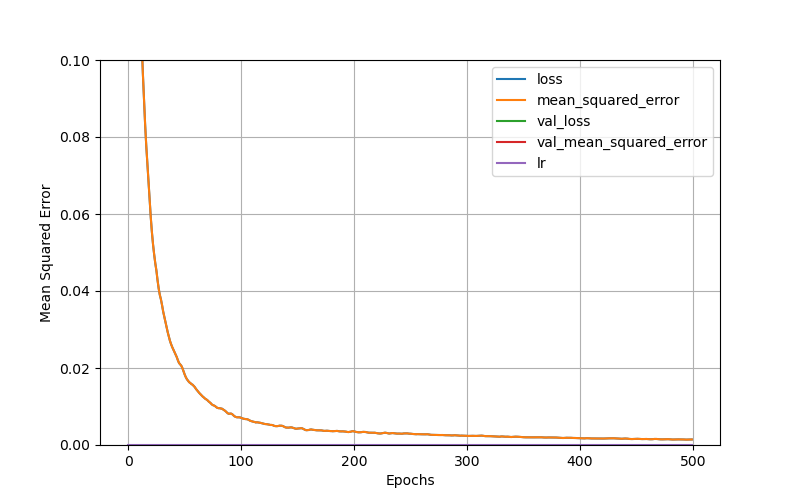
\includegraphics[ width=0.31\textwidth]{psf-CroppedBNFC10000-1-evolution.png}}
		\hspace{\fill}
		\subfloat[Validation example]{%
		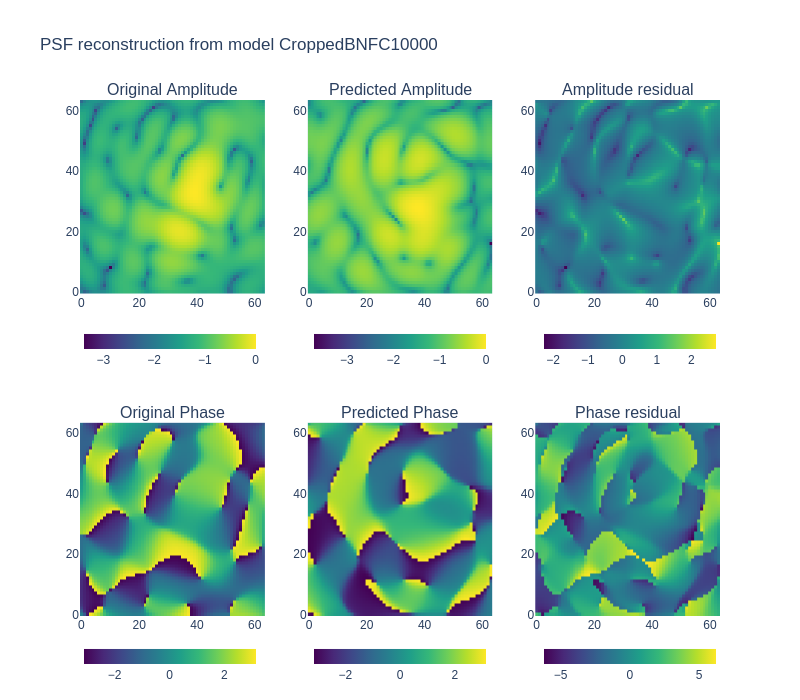
\includegraphics[ width=0.31\textwidth]{psf-CroppedBNFC10000-1-validation.png}}
		\hspace{\fill}
		\subfloat[Train example]{%
		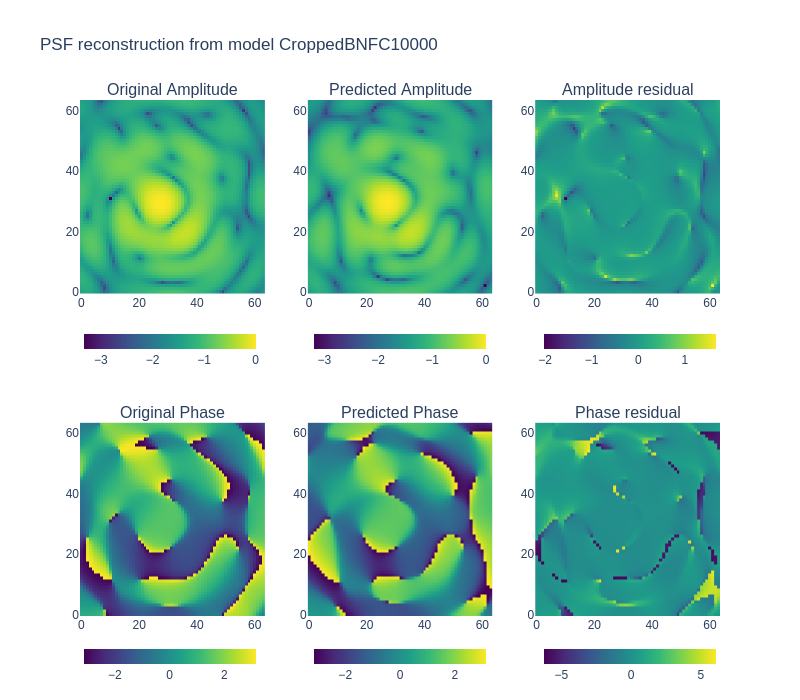
\includegraphics[ width=0.31\textwidth]{psf-CroppedBNFC10000-1-train.png}}\\
		\caption{Results of training the model CroppedBNFC10000-1}
	\end{figure*}
	
\FloatBarrier	
\rule{0.5\textwidth}{0.5pt}\\